\documentclass[a4paper]{article}
\usepackage{listings}    
\usepackage{hyperref}
\usepackage{graphicx} 
\usepackage[T1]{fontenc}
\graphicspath{ {./images/} }   

\begin{document}
\title{Yamaha Aerox Sa14 Limiter Concept}
\author{Kasper Ederzeel, Dylan Duunk}
\date{\today}
\maketitle

\pagenumbering{roman}
\newpage
\tableofcontents
\newpage
\pagenumbering{arabic}

\section{Concept}
We are planning to make a Yamaha Aerox Sa14 Limiter using an Arduino. This is how we are planning to do this: \\
There is running a wire between the CDI and the Pickup Coil which transfers a signal equal to a value in km/h. 
This signal is picked up by an Arduino which checks the signal. \\
If this signal == 0 (or < specified number) the arduino sends a signal equal to a signal of 45km/h to the pickup coil. \\
If this signal is > 0 (or > specified number) the arduino sends the original signal to the pickup coil.
\subsection{Capacitor Discharge Ignition}
What is a CDI System? A Capacitor Discharge Ignition is an
electronic ignition device that stores an electrical 
charge and then discharges it throgh an ignition coil
in order to produce a powerful spark from the spark plugs in a petrol engine.
Here the ignition is provided by the capacitor charge.
The capacitor simply charges and discharges within a fracton of time
making it possible to create sparks. 
\subsubsection{Working principle of an CDI System}
A capacitor discharge ignition works by passing an electrical current over a capacitor.
This type of ignition builds up a charge quickly. 
A CDI ignition starts by generating a charge and storing it up before sending
it out to the spark plug in order to ignite the engine. \\ \\
This power passes through a capacitor and is transferred to an ignition coil that helps
boost the power by acting as a transformer and allowing the energy pass through it instead
of catching any of it. \\ \\
The CDI ignition systems, therefore allow the engine to keep running as long as there is a charge
in the power source. The block diagram of CDI shown below. \\ \\
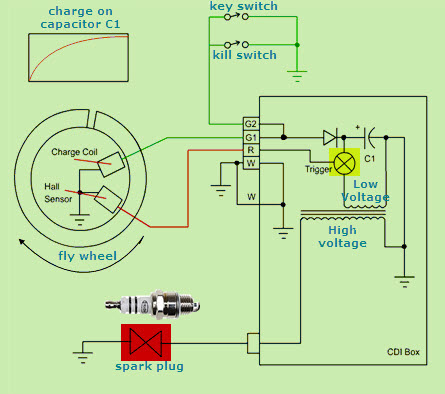
\includegraphics[scale=0.8]{CDI}
\subsubsection{Working of Capacitor Discharge Ignition}
A Capacitor Discharge Ignition consists of several parts and is integrated with the ignition system of
a vehicle. The foremost parts of a CDI include the stator, charging coil, hall sensor, flywheel and the timing mark. \\ \\
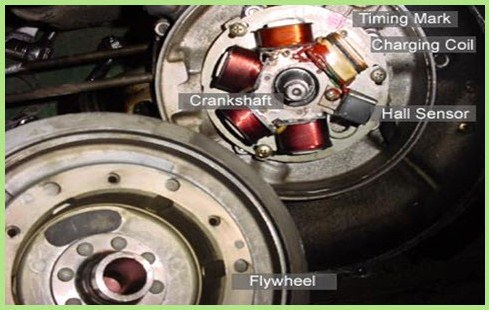
\includegraphics[scale=0.6]{SETUP_CDI}
\subsection{Pickup Coil}
The Pickup Coil is responsible for providing the timing signal to the ignition control box on modern motorcycles
with solid-state ignition systems. The majority of motorcycles from the late 1970's and up use this system for reliable, accurate,
and low maintenance ignition control. On previous models, points-controlled systems were used, and while cheap and simple, they required 
routine maintenance and component replacement to ensure reliability.
\subsubsection{CDI and Solid State Ignition Systems}
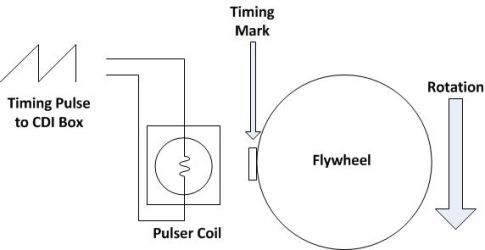
\includegraphics[scale=0.7]{pulser-coil-and-timing} \\ \\
Modern ignition systems use a solid state (semiconductor) controller to handle the ignition spark timing. 
The control box, often called a CDI box, or black box, handles multiple functions. 
The internal electronics are either powered from the battery (DC ignition systems, most street motorcycles), or in AC directly from the stator (most dirt/offroad motorcycles). 
Current from either the stator or the battery is used to charge up an internal capacitor. 
This capacitor is then discharged through the ignition coil via the spark plug to generate the very high voltage necessary for a good spark. 
The CDI box has digitally stored timing maps, to handle advance of the ignition depending on RPM, and sometimes other variables, such as a throttle position sensor (often called TPS, a sensor which varies it's resistance based on the opening of the throttle). 
The CDI box is fed timing data from the Pulser Coil, which produces a short duration, low current, high voltage pulse in relation to the Top Dead Center (TDC) piston location in the engine. 
\end{document}
